\section{Durchführung}
\label{sec:Durchführung}
Damit Dichte, Rauigkeit und Dicke eines Polysterolfilms auf einem Siliziumwafer bestimmt werden können, muss in einem ersten Schritt die Messapparatur
justiert und kalibriert werden.
Der verwendete Versuchsaufbau ist in \autoref{fig:Aufbau} gezeigt, die Datennahme erfolgt über einen angeschlossenen Computer.

\begin{figure}
    \centering
    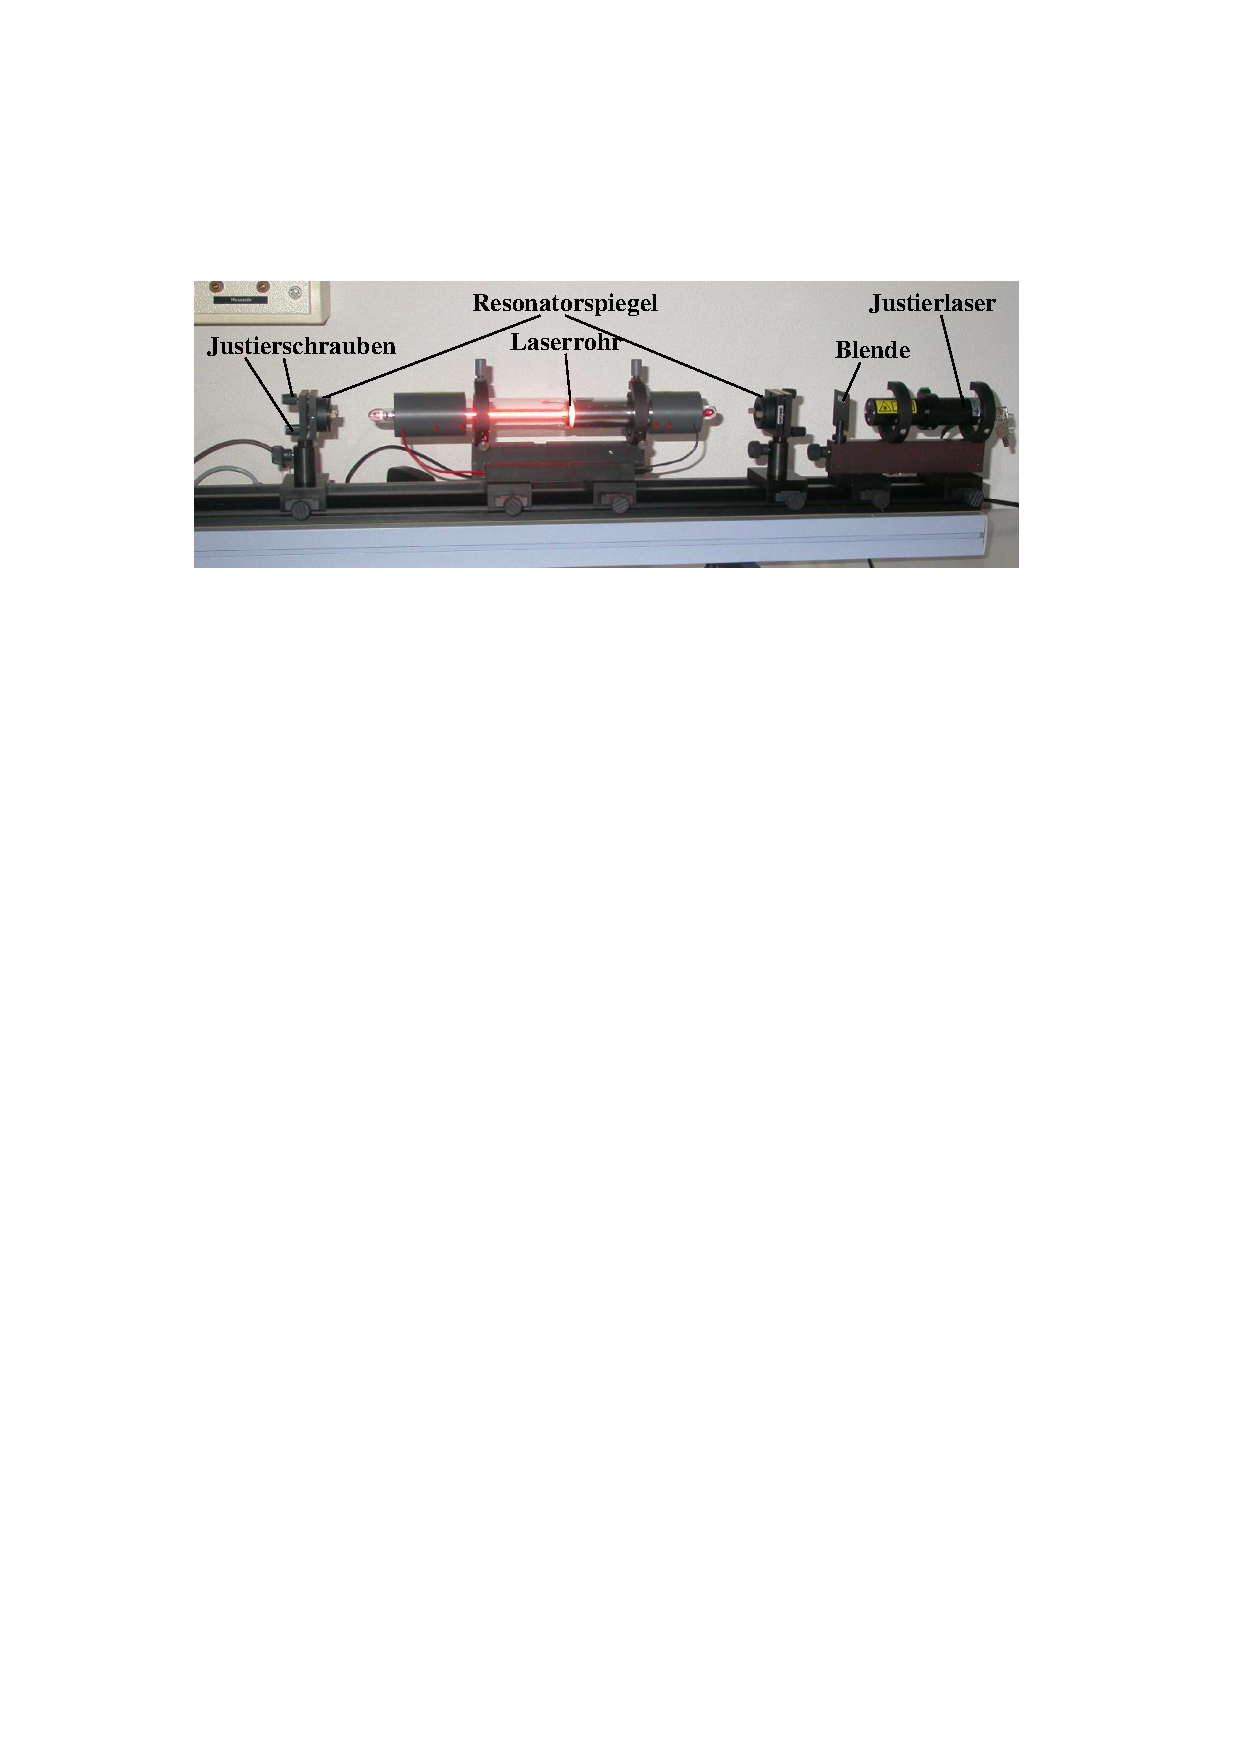
\includegraphics[width=0.9\textwidth]{content/pics/Aufbau.pdf}
    \caption{Bild des verwendeten Diffraktometers. Zu sehen sind \textbf{(a)} Röntgenröhre, \textbf{(b)} Probe, \textbf{(c)} Detektor, \textbf{(d)} xyz-Messtisch.}
    \label{fig:Aufbau}
\end{figure}

\subsection{Justierung der Messapparatur}
Zur Kalibration und Justage werden verschiedene Programme abgefahren. Gestartet wird mit einem Detektorscan, wobei die Probe vollständig aus dem Strahlengang
gefahren wird. Der Detektor wird relativ zur Quelle um einen kleinen Winkel gedreht, sodass der Punkt maximaler Strahlung gefunden werden kann.

Als nächstes wird ein Z-Scan durchgeführt, wobei die Probe in kleine Schritten von unten in den Strahl gefahren wird. Hierbei ist das Ziel, die Einstellung
zu finden, unter der die Probe gerade eben beschienen wird.

Der anschließende X-Scan dient dazu, sicherzustellen, dass die Probe auf der x-Achse richtig plaziert ist.

Darauf folgend wird ein Rockingscan für den Winkel $2\theta = 0$ durchgeführt, der einer Drehung der Probe im Strahlengang entspricht. Hierbei ergibt sich ein Maximum, welches 
der $\qty{0}{\degree}$ Position enspricht.

Abschließend werden ein weiterer Z-Scan, ein Rockingscan für $2\theta = 0,3$, erneut ein Z-Scan und schlussendlich ein letzter Rockingscan für $2\theta = 0,5$ durchgeführt.

Die Messbereiche sind in \autoref{tab:Messbereiche} angegeben. Es ist darauf zu achten, eine angemessene Schrittweite zu verwenden, damit ausreichend viele Daten
vorliegen.

\begin{table}
    \centering
    \caption{Darstellung der zu verwendenden Messbereiche der einzelnen Justagescans.}
    \label{tab:Messbereiche}
    \begin{tabular}{l c}
      \toprule
      {Typ} & {Messbereich} \\
      \midrule
      {Detektorscan}                & {$\numrange{-0,5}{0,5}$}  \\
      {Z-Scan}                      & {$\numrange{-1}{1}$}      \\
      {X-Scan}                      & {$\numrange{-20}{20}$}    \\
      {Rockingscan $2\theta=0$}     & {$\numrange{-1}{1}$}      \\
      {Z-Scan}                      & {$\numrange{-0,5}{0,5}$}  \\
      {Rockingscan $2\theta=0,3$}   & {$\numrange{0}{0,3}$}     \\
      {Z-Scan}                      & {$\numrange{-0,5}{0,5}$}  \\
      {Rockingscan $2\theta=0,3$}   & {$\numrange{0,2}{0,5}$}   \\
      \bottomrule
    \end{tabular}
  \end{table}

\subsection{Vermessung der Probe}
Für einen Messbereich von $\qtyrange{0}{2,5}{\degree}$ wird ein Reflektivscan für den Siliziumwafer durchgeführt. Dabei sind der Einfalls- und Ausfallswinkel 
der Probe gleich. Eine Schrittweite von $\qty{0,005}{\degree}$ mit einer Messdauer vom $\qty{5}{\second}$ ist hierbei einzustellen.

Neben diesem Reflektivscan muss ein Diffuser Scan durchgeführt werden, damit die wahre Reflektivität ermittelt werden kann. Die Schrittweite und Messdauer
soll hierbei identisch zu dem ersten Scan sein, der Detektorwinkel wird jedoch um $\qty{0,1}{\degree}$ gedreht.
Mithilfe der Daten von diesem Scan können die Daten des ersten Scans um etwaige Streueffekte korrigiert werden.